\batchmode

\documentclass[floatfix]{article}
\RequirePackage{ifthen}


\usepackage{graphicx,dcolumn,bm}


\usepackage[dvips]{color}


\pagecolor[gray]{.7}

\usepackage[]{inputenc}



\makeatletter
\AtBeginDocument{\makeatletter
\input C:/cygwin/home/hideaki/05/proj/bec/bec_html/bec.aux
\makeatother
}

\makeatletter
\count@=\the\catcode`\_ \catcode`\_=8 
\newenvironment{tex2html_wrap}{}{}%
\catcode`\<=12\catcode`\_=\count@
\newcommand{\providedcommand}[1]{\expandafter\providecommand\csname #1\endcsname}%
\newcommand{\renewedcommand}[1]{\expandafter\providecommand\csname #1\endcsname{}%
  \expandafter\renewcommand\csname #1\endcsname}%
\newcommand{\newedenvironment}[1]{\newenvironment{#1}{}{}\renewenvironment{#1}}%
\let\newedcommand\renewedcommand
\let\renewedenvironment\newedenvironment
\makeatother
\let\mathon=$
\let\mathoff=$
\ifx\AtBeginDocument\undefined \newcommand{\AtBeginDocument}[1]{}\fi
\newbox\sizebox
\setlength{\hoffset}{0pt}\setlength{\voffset}{0pt}
\addtolength{\textheight}{\footskip}\setlength{\footskip}{0pt}
\addtolength{\textheight}{\topmargin}\setlength{\topmargin}{0pt}
\addtolength{\textheight}{\headheight}\setlength{\headheight}{0pt}
\addtolength{\textheight}{\headsep}\setlength{\headsep}{0pt}
\setlength{\textwidth}{349pt}
\newwrite\lthtmlwrite
\makeatletter
\let\realnormalsize=\normalsize
\global\topskip=2sp
\def\preveqno{}\let\real@float=\@float \let\realend@float=\end@float
\def\@float{\let\@savefreelist\@freelist\real@float}
\def\liih@math{\ifmmode$\else\bad@math\fi}
\def\end@float{\realend@float\global\let\@freelist\@savefreelist}
\let\real@dbflt=\@dbflt \let\end@dblfloat=\end@float
\let\@largefloatcheck=\relax
\let\if@boxedmulticols=\iftrue
\def\@dbflt{\let\@savefreelist\@freelist\real@dbflt}
\def\adjustnormalsize{\def\normalsize{\mathsurround=0pt \realnormalsize
 \parindent=0pt\abovedisplayskip=0pt\belowdisplayskip=0pt}%
 \def\phantompar{\csname par\endcsname}\normalsize}%
\def\lthtmltypeout#1{{\let\protect\string \immediate\write\lthtmlwrite{#1}}}%
\newcommand\lthtmlhboxmathA{\adjustnormalsize\setbox\sizebox=\hbox\bgroup\kern.05em }%
\newcommand\lthtmlhboxmathB{\adjustnormalsize\setbox\sizebox=\hbox to\hsize\bgroup\hfill }%
\newcommand\lthtmlvboxmathA{\adjustnormalsize\setbox\sizebox=\vbox\bgroup %
 \let\ifinner=\iffalse \let\)\liih@math }%
\newcommand\lthtmlboxmathZ{\@next\next\@currlist{}{\def\next{\voidb@x}}%
 \expandafter\box\next\egroup}%
\newcommand\lthtmlmathtype[1]{\gdef\lthtmlmathenv{#1}}%
\newcommand\lthtmllogmath{\lthtmltypeout{l2hSize %
:\lthtmlmathenv:\the\ht\sizebox::\the\dp\sizebox::\the\wd\sizebox.\preveqno}}%
\newcommand\lthtmlfigureA[1]{\let\@savefreelist\@freelist
       \lthtmlmathtype{#1}\lthtmlvboxmathA}%
\newcommand\lthtmlpictureA{\bgroup\catcode`\_=8 \lthtmlpictureB}%
\newcommand\lthtmlpictureB[1]{\lthtmlmathtype{#1}\egroup
       \let\@savefreelist\@freelist \lthtmlhboxmathB}%
\newcommand\lthtmlpictureZ[1]{\hfill\lthtmlfigureZ}%
\newcommand\lthtmlfigureZ{\lthtmlboxmathZ\lthtmllogmath\copy\sizebox
       \global\let\@freelist\@savefreelist}%
\newcommand\lthtmldisplayA{\bgroup\catcode`\_=8 \lthtmldisplayAi}%
\newcommand\lthtmldisplayAi[1]{\lthtmlmathtype{#1}\egroup\lthtmlvboxmathA}%
\newcommand\lthtmldisplayB[1]{\edef\preveqno{(\theequation)}%
  \lthtmldisplayA{#1}\let\@eqnnum\relax}%
\newcommand\lthtmldisplayZ{\lthtmlboxmathZ\lthtmllogmath\lthtmlsetmath}%
\newcommand\lthtmlinlinemathA{\bgroup\catcode`\_=8 \lthtmlinlinemathB}
\newcommand\lthtmlinlinemathB[1]{\lthtmlmathtype{#1}\egroup\lthtmlhboxmathA
  \vrule height1.5ex width0pt }%
\newcommand\lthtmlinlineA{\bgroup\catcode`\_=8 \lthtmlinlineB}%
\newcommand\lthtmlinlineB[1]{\lthtmlmathtype{#1}\egroup\lthtmlhboxmathA}%
\newcommand\lthtmlinlineZ{\egroup\expandafter\ifdim\dp\sizebox>0pt %
  \expandafter\centerinlinemath\fi\lthtmllogmath\lthtmlsetinline}
\newcommand\lthtmlinlinemathZ{\egroup\expandafter\ifdim\dp\sizebox>0pt %
  \expandafter\centerinlinemath\fi\lthtmllogmath\lthtmlsetmath}
\newcommand\lthtmlindisplaymathZ{\egroup %
  \centerinlinemath\lthtmllogmath\lthtmlsetmath}
\def\lthtmlsetinline{\hbox{\vrule width.1em \vtop{\vbox{%
  \kern.1em\copy\sizebox}\ifdim\dp\sizebox>0pt\kern.1em\else\kern.3pt\fi
  \ifdim\hsize>\wd\sizebox \hrule depth1pt\fi}}}
\def\lthtmlsetmath{\hbox{\vrule width.1em\kern-.05em\vtop{\vbox{%
  \kern.1em\kern0.8 pt\hbox{\hglue.17em\copy\sizebox\hglue0.8 pt}}\kern.3pt%
  \ifdim\dp\sizebox>0pt\kern.1em\fi \kern0.8 pt%
  \ifdim\hsize>\wd\sizebox \hrule depth1pt\fi}}}
\def\centerinlinemath{%
  \dimen1=\ifdim\ht\sizebox<\dp\sizebox \dp\sizebox\else\ht\sizebox\fi
  \advance\dimen1by.5pt \vrule width0pt height\dimen1 depth\dimen1 
 \dp\sizebox=\dimen1\ht\sizebox=\dimen1\relax}

\def\lthtmlcheckvsize{\ifdim\ht\sizebox<\vsize 
  \ifdim\wd\sizebox<\hsize\expandafter\hfill\fi \expandafter\vfill
  \else\expandafter\vss\fi}%
\providecommand{\selectlanguage}[1]{}%
\makeatletter \tracingstats = 1 


\begin{document}
\pagestyle{empty}\thispagestyle{empty}\lthtmltypeout{}%
\lthtmltypeout{latex2htmlLength hsize=\the\hsize}\lthtmltypeout{}%
\lthtmltypeout{latex2htmlLength vsize=\the\vsize}\lthtmltypeout{}%
\lthtmltypeout{latex2htmlLength hoffset=\the\hoffset}\lthtmltypeout{}%
\lthtmltypeout{latex2htmlLength voffset=\the\voffset}\lthtmltypeout{}%
\lthtmltypeout{latex2htmlLength topmargin=\the\topmargin}\lthtmltypeout{}%
\lthtmltypeout{latex2htmlLength topskip=\the\topskip}\lthtmltypeout{}%
\lthtmltypeout{latex2htmlLength headheight=\the\headheight}\lthtmltypeout{}%
\lthtmltypeout{latex2htmlLength headsep=\the\headsep}\lthtmltypeout{}%
\lthtmltypeout{latex2htmlLength parskip=\the\parskip}\lthtmltypeout{}%
\lthtmltypeout{latex2htmlLength oddsidemargin=\the\oddsidemargin}\lthtmltypeout{}%
\makeatletter
\if@twoside\lthtmltypeout{latex2htmlLength evensidemargin=\the\evensidemargin}%
\else\lthtmltypeout{latex2htmlLength evensidemargin=\the\oddsidemargin}\fi%
\lthtmltypeout{}%
\makeatother
\setcounter{page}{1}
\onecolumn

% !!! IMAGES START HERE !!!

{\newpage\clearpage
\lthtmlinlinemathA{tex2html_wrap_inline847}%
$n_t(\epsilon _i)$%
\lthtmlinlinemathZ
\lthtmlcheckvsize\clearpage}

{\newpage\clearpage
\lthtmlinlinemathA{tex2html_wrap_inline849}%
$m = 5$%
\lthtmlinlinemathZ
\lthtmlcheckvsize\clearpage}

{\newpage\clearpage
\lthtmlinlinemathA{tex2html_wrap_inline851}%
$T<T_c$%
\lthtmlinlinemathZ
\lthtmlcheckvsize\clearpage}

{\newpage\clearpage
\lthtmlinlinemathA{tex2html_wrap_inline853}%
$T \approx T_c$%
\lthtmlinlinemathZ
\lthtmlcheckvsize\clearpage}

{\newpage\clearpage
\lthtmlinlinemathA{tex2html_wrap_inline855}%
$T>T_c$%
\lthtmlinlinemathZ
\lthtmlcheckvsize\clearpage}

{\newpage\clearpage
\lthtmlinlinemathA{tex2html_wrap_inline857}%
$\alpha $%
\lthtmlinlinemathZ
\lthtmlcheckvsize\clearpage}

{\newpage\clearpage
\lthtmlinlinemathA{tex2html_wrap_inline859}%
$|\alpha |$%
\lthtmlinlinemathZ
\lthtmlcheckvsize\clearpage}

{\newpage\clearpage
\lthtmlinlinemathA{tex2html_wrap_inline865}%
$10$%
\lthtmlinlinemathZ
\lthtmlcheckvsize\clearpage}

{\newpage\clearpage
\lthtmlinlinemathA{tex2html_wrap_inline867}%
$20$%
\lthtmlinlinemathZ
\lthtmlcheckvsize\clearpage}

{\newpage\clearpage
\lthtmlinlinemathA{tex2html_wrap_inline871}%
$T_c \approx 3.33 $%
\lthtmlinlinemathZ
\lthtmlcheckvsize\clearpage}

{\newpage\clearpage
\lthtmlinlinemathA{tex2html_wrap_inline873}%
$6.67 $%
\lthtmlinlinemathZ
\lthtmlcheckvsize\clearpage}

{\newpage\clearpage
\lthtmlinlinemathA{tex2html_wrap_inline875}%
$13.3 $%
\lthtmlinlinemathZ
\lthtmlcheckvsize\clearpage}

{\newpage\clearpage
\lthtmlinlinemathA{tex2html_wrap_inline877}%
$T_c$%
\lthtmlinlinemathZ
\lthtmlcheckvsize\clearpage}

{\newpage\clearpage
\lthtmlinlinemathA{tex2html_wrap_inline879}%
$\sigma $%
\lthtmlinlinemathZ
\lthtmlcheckvsize\clearpage}

{\newpage\clearpage
\lthtmlinlinemathA{tex2html_wrap_inline881}%
$m = 20$%
\lthtmlinlinemathZ
\lthtmlcheckvsize\clearpage}

{\newpage\clearpage
\lthtmlinlinemathA{tex2html_wrap_inline883}%
$ \varphi _t (\epsilon _{\mathop {\mathgroup \symoperators min}}) / \sum \nolimits _j \varphi _t (\epsilon _j) $%
\lthtmlinlinemathZ
\lthtmlcheckvsize\clearpage}

{\newpage\clearpage
\lthtmlinlinemathA{tex2html_wrap_inline885}%
$t = 200$%
\lthtmlinlinemathZ
\lthtmlcheckvsize\clearpage}

{\newpage\clearpage
\lthtmlinlinemathA{tex2html_wrap_inline889}%
$y_0 = 1 $%
\lthtmlinlinemathZ
\lthtmlcheckvsize\clearpage}

{\newpage\clearpage
\lthtmlinlinemathA{tex2html_wrap_inline891}%
$l = 1$%
\lthtmlinlinemathZ
\lthtmlcheckvsize\clearpage}

{\newpage\clearpage
\lthtmlinlinemathA{tex2html_wrap_inline893}%
$\sigma = 3$%
\lthtmlinlinemathZ
\lthtmlcheckvsize\clearpage}

{\newpage\clearpage
\lthtmlinlinemathA{tex2html_wrap_inline895}%
$\epsilon _{\mathop {\mathgroup \symoperators max}} = 1$%
\lthtmlinlinemathZ
\lthtmlcheckvsize\clearpage}

{\newpage\clearpage
\lthtmlinlinemathA{tex2html_wrap_inline922}%
$\mathaccent "707E\relax {m}=100$%
\lthtmlinlinemathZ
\lthtmlcheckvsize\clearpage}

{\newpage\clearpage
\lthtmlinlinemathA{tex2html_wrap_inline924}%
$100$%
\lthtmlinlinemathZ
\lthtmlcheckvsize\clearpage}

{\newpage\clearpage
\lthtmlinlinemathA{tex2html_wrap_inline926}%
$T=1$%
\lthtmlinlinemathZ
\lthtmlcheckvsize\clearpage}

{\newpage\clearpage
\lthtmlinlinemathA{tex2html_wrap_inline928}%
$\sigma = 3/2$%
\lthtmlinlinemathZ
\lthtmlcheckvsize\clearpage}

{\newpage\clearpage
\lthtmlinlinemathA{tex2html_wrap_inline932}%
$i$%
\lthtmlinlinemathZ
\lthtmlcheckvsize\clearpage}

{\newpage\clearpage
\lthtmlinlinemathA{tex2html_wrap_inline934}%
$\eta = 0.01$%
\lthtmlinlinemathZ
\lthtmlcheckvsize\clearpage}

{\newpage\clearpage
\lthtmlinlinemathA{tex2html_wrap_inline936}%
$T_i$%
\lthtmlinlinemathZ
\lthtmlcheckvsize\clearpage}

{\newpage\clearpage
\lthtmlinlinemathA{tex2html_wrap_inline938}%
$\gamma = 2$%
\lthtmlinlinemathZ
\lthtmlcheckvsize\clearpage}

{\newpage\clearpage
\lthtmlinlinemathA{tex2html_wrap_inline940}%
$T_c = 33$%
\lthtmlinlinemathZ
\lthtmlcheckvsize\clearpage}


%
\providecommand{\figref}[1]{FIG.~\ref{#1}}%


%
\providecommand{\Eq}[1]{Eq.~\ref{#1}}%

{\newpage\clearpage
\lthtmlinlinemathA{tex2html_wrap_inline309}%
$\varphi(\epsilon)$%
\lthtmlinlinemathZ
\lthtmlcheckvsize\clearpage}

{\newpage\clearpage
\lthtmlinlinemathA{tex2html_wrap_inline311}%
$C^2$%
\lthtmlinlinemathZ
\lthtmlcheckvsize\clearpage}

{\newpage\clearpage
\lthtmlinlinemathA{tex2html_wrap_inline313}%
$g(\epsilon ) (\geq 0)$%
\lthtmlinlinemathZ
\lthtmlcheckvsize\clearpage}

{\newpage\clearpage
\lthtmlinlinemathA{tex2html_wrap_inline315}%
$\epsilon \in [0,\epsilon_{\max}]$%
\lthtmlinlinemathZ
\lthtmlcheckvsize\clearpage}

{\newpage\clearpage
\lthtmlinlinemathA{tex2html_wrap_indisplay958}%
$\displaystyle \int{d\epsilon \, g(\epsilon)}$%
\lthtmlindisplaymathZ
\lthtmlcheckvsize\clearpage}

{\newpage\clearpage
\lthtmlinlinemathA{tex2html_wrap_indisplay959}%
$\textstyle =$%
\lthtmlindisplaymathZ
\lthtmlcheckvsize\clearpage}

{\newpage\clearpage
\lthtmlinlinemathA{tex2html_wrap_indisplay960}%
$\displaystyle 1,$%
\lthtmlindisplaymathZ
\lthtmlcheckvsize\clearpage}

{\newpage\clearpage
\lthtmlinlinemathA{tex2html_wrap_indisplay961}%
$\displaystyle \int{d\epsilon \, g(\epsilon)\varphi (\epsilon)}$%
\lthtmlindisplaymathZ
\lthtmlcheckvsize\clearpage}

{\newpage\clearpage
\lthtmlinlinemathA{tex2html_wrap_indisplay963}%
$\displaystyle m + y_0,$%
\lthtmlindisplaymathZ
\lthtmlcheckvsize\clearpage}

{\newpage\clearpage
\lthtmlinlinemathA{tex2html_wrap_indisplay964}%
$\displaystyle \int{d\epsilon \, g(\epsilon)e^{- \beta \epsilon} \varphi(\epsilon)}$%
\lthtmlindisplaymathZ
\lthtmlcheckvsize\clearpage}

{\newpage\clearpage
\lthtmlinlinemathA{tex2html_wrap_indisplay966}%
$\displaystyle M.$%
\lthtmlindisplaymathZ
\lthtmlcheckvsize\clearpage}

{\newpage\clearpage
\lthtmlinlinemathA{tex2html_wrap_inline317}%
$\beta$%
\lthtmlinlinemathZ
\lthtmlcheckvsize\clearpage}

{\newpage\clearpage
\lthtmldisplayA{displaymath242}%
\begin{displaymath}
\varphi(\epsilon) = \frac{y_0}{1 - e^{-\beta \epsilon
- \alpha}}, \end{displaymath}%
\lthtmldisplayZ
\lthtmlcheckvsize\clearpage}

{\newpage\clearpage
\lthtmlinlinemathA{tex2html_wrap_inline321}%
$e^{-\alpha}=m/M$%
\lthtmlinlinemathZ
\lthtmlcheckvsize\clearpage}

{\newpage\clearpage
\lthtmlinlinemathA{tex2html_wrap_inline323}%
$y_0$%
\lthtmlinlinemathZ
\lthtmlcheckvsize\clearpage}

{\newpage\clearpage
\lthtmldisplayA{displaymath246}%
\begin{displaymath}
\int
{d\epsilon \, g(\epsilon)\frac{\varphi(\epsilon) - y_0}{y_0} } = N,
\end{displaymath}%
\lthtmldisplayZ
\lthtmlcheckvsize\clearpage}

{\newpage\clearpage
\lthtmlinlinemathA{tex2html_wrap_inline325}%
$N = m/y_0$%
\lthtmlinlinemathZ
\lthtmlcheckvsize\clearpage}

{\newpage\clearpage
\lthtmlinlinemathA{tex2html_wrap_inline327}%
$ N/M$%
\lthtmlinlinemathZ
\lthtmlcheckvsize\clearpage}

{\newpage\clearpage
\lthtmldisplayA{displaymath252}%
\begin{displaymath}
n(\epsilon) = \frac{\varphi(\epsilon) - y_0}{y_0} =
\frac{1}{e^{\beta \epsilon + \alpha} - 1}, \end{displaymath}%
\lthtmldisplayZ
\lthtmlcheckvsize\clearpage}

{\newpage\clearpage
\lthtmlinlinemathA{tex2html_wrap_inline331}%
$e^{-\beta \epsilon - \alpha}<1$%
\lthtmlinlinemathZ
\lthtmlcheckvsize\clearpage}

{\newpage\clearpage
\lthtmldisplayA{displaymath255}%
\begin{displaymath}
y_i(t+1) = a_i b(t)y_i(t),
\end{displaymath}%
\lthtmldisplayZ
\lthtmlcheckvsize\clearpage}

{\newpage\clearpage
\lthtmlinlinemathA{tex2html_wrap_inline333}%
$y_i(t)$%
\lthtmlinlinemathZ
\lthtmlcheckvsize\clearpage}

{\newpage\clearpage
\lthtmlinlinemathA{tex2html_wrap_inline337}%
$t$%
\lthtmlinlinemathZ
\lthtmlcheckvsize\clearpage}

{\newpage\clearpage
\lthtmlinlinemathA{tex2html_wrap_inline339}%
$a_i$%
\lthtmlinlinemathZ
\lthtmlcheckvsize\clearpage}

{\newpage\clearpage
\lthtmlinlinemathA{tex2html_wrap_inline341}%
$\rho(a)$%
\lthtmlinlinemathZ
\lthtmlcheckvsize\clearpage}

{\newpage\clearpage
\lthtmlinlinemathA{tex2html_wrap_inline343}%
$b(t)$%
\lthtmlinlinemathZ
\lthtmlcheckvsize\clearpage}

{\newpage\clearpage
\lthtmlinlinemathA{tex2html_wrap_inline345}%
$l$%
\lthtmlinlinemathZ
\lthtmlcheckvsize\clearpage}

{\newpage\clearpage
\lthtmlinlinemathA{tex2html_wrap_inline347}%
$t
+ 1 $%
\lthtmlinlinemathZ
\lthtmlcheckvsize\clearpage}

{\newpage\clearpage
\lthtmlinlinemathA{tex2html_wrap_inline349}%
$(i=0, \cdots, t)$%
\lthtmlinlinemathZ
\lthtmlcheckvsize\clearpage}

{\newpage\clearpage
\lthtmlinlinemathA{tex2html_wrap_inline353}%
$b(t) =
m/M_t$%
\lthtmlinlinemathZ
\lthtmlcheckvsize\clearpage}

{\newpage\clearpage
\lthtmlinlinemathA{tex2html_wrap_inline355}%
$M_t$%
\lthtmlinlinemathZ
\lthtmlcheckvsize\clearpage}

{\newpage\clearpage
\lthtmldisplayA{displaymath257}%
\begin{displaymath}
M_t = \sum\limits_{j = 0}^t {a_j y_j (t)}.
\end{displaymath}%
\lthtmldisplayZ
\lthtmlcheckvsize\clearpage}

{\newpage\clearpage
\lthtmlinlinemathA{tex2html_wrap_inline361}%
$m $%
\lthtmlinlinemathZ
\lthtmlcheckvsize\clearpage}

{\newpage\clearpage
\lthtmlinlinemathA{tex2html_wrap_inline363}%
$t > 0$%
\lthtmlinlinemathZ
\lthtmlcheckvsize\clearpage}

{\newpage\clearpage
\lthtmlinlinemathA{tex2html_wrap_inline365}%
$y_i(i) = y_0$%
\lthtmlinlinemathZ
\lthtmlcheckvsize\clearpage}

{\newpage\clearpage
\lthtmlinlinemathA{tex2html_wrap_inline367}%
$y_0(0)=m + y_0$%
\lthtmlinlinemathZ
\lthtmlcheckvsize\clearpage}

{\newpage\clearpage
\lthtmlinlinemathA{tex2html_wrap_inline369}%
$m + y_0 $%
\lthtmlinlinemathZ
\lthtmlcheckvsize\clearpage}

{\newpage\clearpage
\lthtmlinlinemathA{tex2html_wrap_inline371}%
$a \in [a_{\min},1]$%
\lthtmlinlinemathZ
\lthtmlcheckvsize\clearpage}

{\newpage\clearpage
\lthtmlinlinemathA{tex2html_wrap_inline373}%
$a_{\min}> 0$%
\lthtmlinlinemathZ
\lthtmlcheckvsize\clearpage}

{\newpage\clearpage
\lthtmlinlinemathA{tex2html_wrap_inline379}%
$y_i(t)=\Omega_i(t) y_0$%
\lthtmlinlinemathZ
\lthtmlcheckvsize\clearpage}

{\newpage\clearpage
\lthtmldisplayA{displaymath259}%
\begin{displaymath}
\Omega _i(t) = a_i^{t-i}
\left( \prod\limits_{t'=i}^{t - 1}{b(t')} \right).  \end{displaymath}%
\lthtmldisplayZ
\lthtmlcheckvsize\clearpage}

{\newpage\clearpage
\lthtmlinlinemathA{tex2html_wrap_inline381}%
$\Omega_i(t)$%
\lthtmlinlinemathZ
\lthtmlcheckvsize\clearpage}

{\newpage\clearpage
\lthtmlinlinemathA{tex2html_wrap_inline385}%
$\beta (=1/T) $%
\lthtmlinlinemathZ
\lthtmlcheckvsize\clearpage}

{\newpage\clearpage
\lthtmlinlinemathA{tex2html_wrap_inline387}%
$a = e^{ - \beta
\epsilon }$%
\lthtmlinlinemathZ
\lthtmlcheckvsize\clearpage}

{\newpage\clearpage
\lthtmlinlinemathA{tex2html_wrap_inline391}%
$g(
\epsilon )$%
\lthtmlinlinemathZ
\lthtmlcheckvsize\clearpage}

{\newpage\clearpage
\lthtmlinlinemathA{tex2html_wrap_inline393}%
$\rho(a) \left( = g(\epsilon)\left|
{{\textstyle{{d\epsilon } \over {da}}}} \right| \right)$%
\lthtmlinlinemathZ
\lthtmlcheckvsize\clearpage}

{\newpage\clearpage
\lthtmldisplayA{displaymath262}%
\begin{displaymath}
\ln \Omega_i = (t-i)\left\{-
\beta \epsilon_i - \left\langle {\ln b} \right\rangle \right\}, \end{displaymath}%
\lthtmldisplayZ
\lthtmlcheckvsize\clearpage}

{\newpage\clearpage
\lthtmlinlinemathA{tex2html_wrap_inline401}%
$\ln \prod\nolimits_{t'=i}^{t - 1} {b( t' )} = \sum\nolimits_{t'
= i}^{t - 1} {\ln b( t' )} \sim (t -i) \left\langle {\ln b}
\right\rangle$%
\lthtmlinlinemathZ
\lthtmlcheckvsize\clearpage}

{\newpage\clearpage
\lthtmldisplayA{displaymath264}%
\begin{displaymath}
\left\langle {\ln b} \right\rangle = -\alpha,
\end{displaymath}%
\lthtmldisplayZ
\lthtmlcheckvsize\clearpage}

{\newpage\clearpage
\lthtmlinlinemathA{tex2html_wrap_inline407}%
$y_i(t) =
e^{(-\beta \epsilon_i - \alpha)(t-i)} y_0 $%
\lthtmlinlinemathZ
\lthtmlcheckvsize\clearpage}

{\newpage\clearpage
\lthtmlinlinemathA{tex2html_wrap_inline409}%
$e^{-\beta
\epsilon_i - \alpha} < 1$%
\lthtmlinlinemathZ
\lthtmlcheckvsize\clearpage}

{\newpage\clearpage
\lthtmlinlinemathA{tex2html_wrap_inline411}%
$\varphi_t (\epsilon_i)
= \sum\nolimits_{t' = i}^t {y_i ( {t'} )} $%
\lthtmlinlinemathZ
\lthtmlcheckvsize\clearpage}

{\newpage\clearpage
\lthtmlinlinemathA{tex2html_wrap_inline413}%
$\varphi (
\epsilon_i )$%
\lthtmlinlinemathZ
\lthtmlcheckvsize\clearpage}

{\newpage\clearpage
\lthtmlinlinemathA{tex2html_wrap_inline415}%
$\varphi _t
(\epsilon_i )$%
\lthtmlinlinemathZ
\lthtmlcheckvsize\clearpage}

{\newpage\clearpage
\lthtmlinlinemathA{tex2html_wrap_inline419}%
$n_t ( \epsilon_i  ) = \{\varphi_t (\epsilon_i) - y_0\}/{y_0}$%
\lthtmlinlinemathZ
\lthtmlcheckvsize\clearpage}

{\newpage\clearpage
\lthtmlinlinemathA{tex2html_wrap_inline421}%
$(t \to
\infty)$%
\lthtmlinlinemathZ
\lthtmlcheckvsize\clearpage}

{\newpage\clearpage
\lthtmldisplayA{displaymath269}%
\begin{displaymath}
\mathop {\lim }\limits_{t \to \infty } M_t = \int {d\epsilon \,
g(\epsilon)\sum\limits_{t'=0}^\infty {e^{- \beta \epsilon} y(t')} },
\end{displaymath}%
\lthtmldisplayZ
\lthtmlcheckvsize\clearpage}

{\newpage\clearpage
\lthtmlinlinemathA{tex2html_wrap_inline423}%
$\sum\nolimits_{t'=0}^\infty y(t') = \varphi(\epsilon)$%
\lthtmlinlinemathZ
\lthtmlcheckvsize\clearpage}

{\newpage\clearpage
\lthtmlinlinemathA{tex2html_wrap_inline425}%
$\mathop {\lim }\limits_{t \to
\infty } \ln b( t ) = \left\langle {\ln b} \right\rangle $%
\lthtmlinlinemathZ
\lthtmlcheckvsize\clearpage}

{\newpage\clearpage
\lthtmlinlinemathA{tex2html_wrap_inline427}%
$\mathop
{\lim }\limits_{t \to \infty } {m \mathord{\left/ \right.} {M_t }} = e^{ -
\alpha } $%
\lthtmlinlinemathZ
\lthtmlcheckvsize\clearpage}

{\newpage\clearpage
\lthtmldisplayA{displaymath273}%
\begin{displaymath}
\int {d\epsilon \, g(\epsilon)\frac{1}{e^{\beta \epsilon + \alpha } - 1}} =
N,
\end{displaymath}%
\lthtmldisplayZ
\lthtmlcheckvsize\clearpage}

{\newpage\clearpage
\lthtmlinlinemathA{tex2html_wrap_inline431}%
$l (\geq 1)$%
\lthtmlinlinemathZ
\lthtmlcheckvsize\clearpage}

{\newpage\clearpage
\lthtmlinlinemathA{tex2html_wrap_inline435}%
$N = m / y_0 l$%
\lthtmlinlinemathZ
\lthtmlcheckvsize\clearpage}

{\newpage\clearpage
\lthtmldisplayA{displaymath279}%
\begin{displaymath}
g(\epsilon) = C_\sigma \epsilon^{\sigma-1}, \end{displaymath}%
\lthtmldisplayZ
\lthtmlcheckvsize\clearpage}

{\newpage\clearpage
\lthtmlinlinemathA{tex2html_wrap_inline441}%
$C_\sigma =
\sigma / \epsilon_{\max}^\sigma$%
\lthtmlinlinemathZ
\lthtmlcheckvsize\clearpage}

{\newpage\clearpage
\lthtmlinlinemathA{tex2html_wrap_inline443}%
$(\sigma>1)$%
\lthtmlinlinemathZ
\lthtmlcheckvsize\clearpage}

{\newpage\clearpage
\lthtmlinlinemathA{tex2html_wrap_inline447}%
$T$%
\lthtmlinlinemathZ
\lthtmlcheckvsize\clearpage}

{\newpage\clearpage
\lthtmlinlinemathA{tex2html_wrap_inline453}%
$\alpha=0$%
\lthtmlinlinemathZ
\lthtmlcheckvsize\clearpage}

{\newpage\clearpage
\lthtmlinlinemathA{tex2html_wrap_inline459}%
$\epsilon_i < -\alpha / \beta$%
\lthtmlinlinemathZ
\lthtmlcheckvsize\clearpage}

{\newpage\clearpage
\lthtmlinlinemathA{tex2html_wrap_inline461}%
$y = \beta \epsilon $%
\lthtmlinlinemathZ
\lthtmlcheckvsize\clearpage}

{\newpage\clearpage
\lthtmldisplayA{displaymath284}%
\begin{displaymath}
N = \frac{\sigma
}{(\beta \epsilon_{\max})^\sigma} \int_0^{\beta \epsilon _{\max} }
{\frac{{y^{\sigma - 1} }}{e^y - 1} \,dy}.  \end{displaymath}%
\lthtmldisplayZ
\lthtmlcheckvsize\clearpage}

{\newpage\clearpage
\lthtmlinlinemathA{tex2html_wrap_inline465}%
$T_c({ = 1/\beta _c })$%
\lthtmlinlinemathZ
\lthtmlcheckvsize\clearpage}

{\newpage\clearpage
\lthtmldisplayA{displaymath287}%
\begin{displaymath}
T_c^{( 1
)} \sim \epsilon _{\max} \left\{ {N^{ - 1} \Gamma(\sigma + 1)
\zeta(\sigma)} \right\}^{ - {\textstyle{\frac{1}{\sigma} }}}, \end{displaymath}%
\lthtmldisplayZ
\lthtmlcheckvsize\clearpage}

{\newpage\clearpage
\lthtmlinlinemathA{tex2html_wrap_inline467}%
$N \ll 1$%
\lthtmlinlinemathZ
\lthtmlcheckvsize\clearpage}

{\newpage\clearpage
\lthtmlinlinemathA{tex2html_wrap_inline469}%
$N \gg 1$%
\lthtmlinlinemathZ
\lthtmlcheckvsize\clearpage}

{\newpage\clearpage
\lthtmlinlinemathA{tex2html_wrap_inline471}%
$e^y \simeq 1 +
y$%
\lthtmlinlinemathZ
\lthtmlcheckvsize\clearpage}

{\newpage\clearpage
\lthtmldisplayA{displaymath290}%
\begin{displaymath}
T_c^{(2)} \sim
\epsilon_{\max}(1 - \sigma^{-1}) N.  \end{displaymath}%
\lthtmldisplayZ
\lthtmlcheckvsize\clearpage}

{\newpage\clearpage
\lthtmlinlinemathA{tex2html_wrap_inline473}%
${\varphi_t
(\epsilon_{\min})} \mathord{\left/ {\sum\nolimits_j {\varphi_t (
{\epsilon_j } )} } \right.} $%
\lthtmlinlinemathZ
\lthtmlcheckvsize\clearpage}

{\newpage\clearpage
\lthtmlinlinemathA{tex2html_wrap_inline515}%
$ \varphi_t (\epsilon _{\min}) / \sum\nolimits_j
\varphi_t (\epsilon _j) $%
\lthtmlinlinemathZ
\lthtmlcheckvsize\clearpage}

{\newpage\clearpage
\lthtmlinlinemathA{tex2html_wrap_inline527}%
$\epsilon
_{\max } = 1$%
\lthtmlinlinemathZ
\lthtmlcheckvsize\clearpage}

{\newpage\clearpage
\lthtmlpictureA{tex2html_wrap1115}%
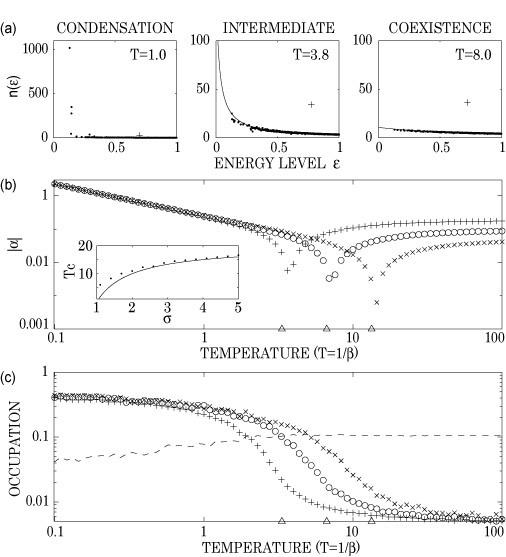
\includegraphics[width=8.7cm]{FIG1}%
\lthtmlpictureZ
\lthtmlcheckvsize\clearpage}

{\newpage\clearpage
\lthtmlinlinemathA{tex2html_wrap_inline535}%
$M_t/(m+y_0)$%
\lthtmlinlinemathZ
\lthtmlcheckvsize\clearpage}

{\newpage\clearpage
\lthtmlinlinemathA{tex2html_wrap_inline541}%
$\eta$%
\lthtmlinlinemathZ
\lthtmlcheckvsize\clearpage}

{\newpage\clearpage
\lthtmlinlinemathA{tex2html_wrap_inline545}%
$y_i(t+1)$%
\lthtmlinlinemathZ
\lthtmlcheckvsize\clearpage}

{\newpage\clearpage
\lthtmlinlinemathA{tex2html_wrap_inline547}%
$i = 1, \cdots, Q(t)$%
\lthtmlinlinemathZ
\lthtmlcheckvsize\clearpage}

{\newpage\clearpage
\lthtmlinlinemathA{tex2html_wrap_inline549}%
$  \lambda_i = \tilde{m} \frac { (1-\eta) a_i y_i(t) }{\sum_{i=0}^{Q(t)}
{ a_i y_i(t)} }.$%
\lthtmlinlinemathZ
\lthtmlcheckvsize\clearpage}

{\newpage\clearpage
\lthtmlinlinemathA{tex2html_wrap_inline551}%
$Q(t)$%
\lthtmlinlinemathZ
\lthtmlcheckvsize\clearpage}

{\newpage\clearpage
\lthtmlinlinemathA{tex2html_wrap_inline555}%
$Q(t+1)-Q(t)$%
\lthtmlinlinemathZ
\lthtmlcheckvsize\clearpage}

{\newpage\clearpage
\lthtmlinlinemathA{tex2html_wrap_inline557}%
$ l = \tilde{m} \frac { \sum_{j=0}^{Q(t)} {\eta a_j y_j(t)} } {
\sum_{i=0}^{Q(t)} { a_i y_i(t)} }$%
\lthtmlinlinemathZ
\lthtmlcheckvsize\clearpage}

{\newpage\clearpage
\lthtmlinlinemathA{tex2html_wrap_inline561}%
$\sum_{i=0}^{Q(t)} \lambda_i + l = \tilde{m}$%
\lthtmlinlinemathZ
\lthtmlcheckvsize\clearpage}

{\newpage\clearpage
\lthtmlinlinemathA{tex2html_wrap_inline569}%
$ a \in [0,1]$%
\lthtmlinlinemathZ
\lthtmlcheckvsize\clearpage}

{\newpage\clearpage
\lthtmlinlinemathA{tex2html_wrap_inline583}%
$N$%
\lthtmlinlinemathZ
\lthtmlcheckvsize\clearpage}

{\newpage\clearpage
\lthtmlinlinemathA{tex2html_wrap_inline585}%
$\eta = {l} /(m + l) = (N + 1)^{-1}$%
\lthtmlinlinemathZ
\lthtmlcheckvsize\clearpage}

{\newpage\clearpage
\lthtmldisplayA{displaymath302}%
\begin{displaymath}
T_c \sim \epsilon_{\max}(1-\sigma^{-1}) ( \eta^{-1} - 1). \end{displaymath}%
\lthtmldisplayZ
\lthtmlcheckvsize\clearpage}

{\newpage\clearpage
\lthtmlinlinemathA{tex2html_wrap_inline595}%
$\tilde{m}=100$%
\lthtmlinlinemathZ
\lthtmlcheckvsize\clearpage}

{\newpage\clearpage
\lthtmlpictureA{tex2html_wrap1173}%
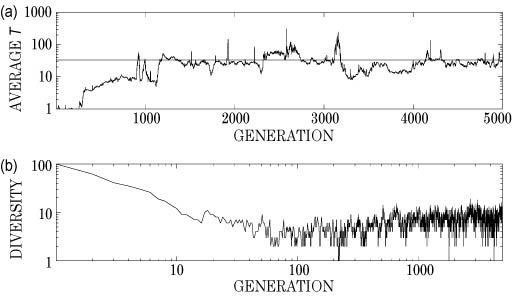
\includegraphics[width=8.7cm]{FIG2}%
\lthtmlpictureZ
\lthtmlcheckvsize\clearpage}

{\newpage\clearpage
\lthtmlinlinemathA{tex2html_wrap_inline629}%
$T_i = 1/\beta_i$%
\lthtmlinlinemathZ
\lthtmlcheckvsize\clearpage}

{\newpage\clearpage
\lthtmlinlinemathA{tex2html_wrap_inline631}%
$\beta_i$%
\lthtmlinlinemathZ
\lthtmlcheckvsize\clearpage}

{\newpage\clearpage
\lthtmlinlinemathA{tex2html_wrap_inline635}%
$\left\langle
a \right\rangle = e^{ - \beta_i \left\langle \varepsilon
\right\rangle }< a_i$%
\lthtmlinlinemathZ
\lthtmlcheckvsize\clearpage}

{\newpage\clearpage
\lthtmlinlinemathA{tex2html_wrap_inline637}%
$\left\langle \varepsilon \right\rangle
= \varepsilon _{\max } {\sigma \mathord{\left/ {\vphantom {\sigma
{\left( {\sigma + 1} \right)}}} \right.  \kern-\nulldelimiterspace}
{\left( {\sigma + 1} \right)}}$%
\lthtmlinlinemathZ
\lthtmlcheckvsize\clearpage}

{\newpage\clearpage
\lthtmldisplayA{displaymath306}%
\begin{displaymath}
\beta _i = - \gamma \left\langle \varepsilon
\right\rangle ^{ - 1} \ln a_i, \end{displaymath}%
\lthtmldisplayZ
\lthtmlcheckvsize\clearpage}

{\newpage\clearpage
\lthtmlinlinemathA{tex2html_wrap_inline641}%
$\gamma > 1$%
\lthtmlinlinemathZ
\lthtmlcheckvsize\clearpage}

{\newpage\clearpage
\lthtmlinlinemathA{tex2html_wrap_inline643}%
$\left\langle a \right\rangle < a_i$%
\lthtmlinlinemathZ
\lthtmlcheckvsize\clearpage}


\end{document}
